\documentclass{article}
\graphicspath{{/home/david/Book/Chapters/2.Vectors/Vectors/pic/}}

% !TeX root = ../../../Mainfile/book.tex



\begin{document}


\color{white}\subsection{Vector properties}\color{black}


\begin{minipage}{0.1\textwidth}
\quad
\end{minipage}
\begin{minipage}{0.25\textwidth}
\begin{align*}
\vec{v}  = \color{rooj} \begin{bmatrix} 4 & 3 \end{bmatrix}  \color{black}
 =  \color{groen} \begin{bmatrix} 4 \\ 3 \end{bmatrix}  \color{black}
\end{align*}
\end{minipage} \hfill
\begin{minipage}{0.4\textwidth}
\begin{figure}[H]
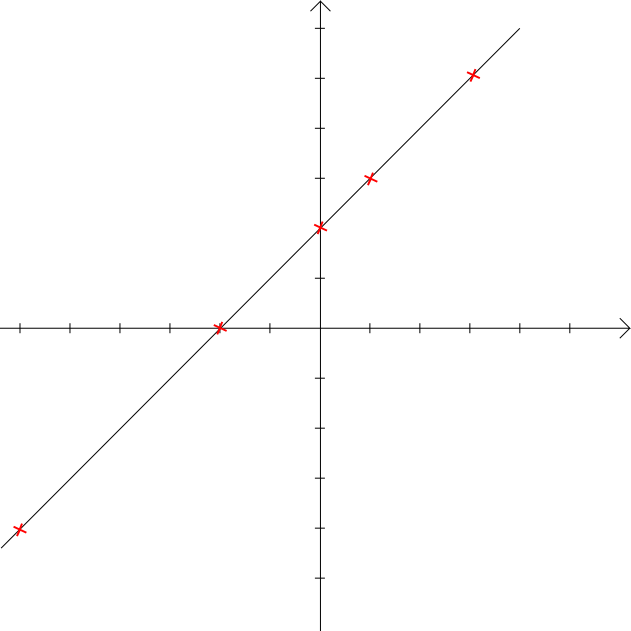
\includegraphics[width = 0.9\linewidth]{1.png}
\end{figure}
\end{minipage}
\begin{minipage}{0.1\textwidth}
\quad
\end{minipage}

\

\paragraph{Vectors: } Its easy to think of vectors as a \textbf{length} and a \textbf{direction}, usually denoted $v = [x_1  x_2  x_3  \dots  x_n]$.

\

Above we have an example of  a (\textbf{2-dimensional}) vector, written both as a \color{rooj} row vector \color{black} and a \color{groen} column vector\color{black}. The vector represents a "travel" by 4 steps along the $x_1$ axis and 3 steps along the $x_2$ axis. So if you find yourself positioned at the point $(2,-4)$ and someone "applies" this vector to you, you'll be moved to $(2+4, -4+3) = (6,-1)$.

\paragraph{Vector operations: }


The length of a vector is written as $|\vec{v}|$ and found with the Pythagorean-theorem:

\[
|\vec{v}| = \sqrt{4^2 + 3^2} = \sqrt{25} = 5
\]

and its direction is written $\theta_{\vec{v}}$ and calculated using absolute classic geometry

\[
\theta_{\vec{v}} = \tan^{-1}\frac{3}{4} 
\]

To \textbf{transpose} a vector, $\vec{v^T}$ is simply to change it from a \color{rooj} row vector \color{black} to a \color{groen} column vector \color{black} and vice-versa

\begin{align*}
\begin{bmatrix} 4 & 3 \end{bmatrix}^T   =  \begin{bmatrix} 4 \\ 3 \end{bmatrix} 
\end{align*}

\paragraph{Example: }

\paragraph{Exercise: } asd



\end{document}